\chapter{Anforderungsanalyse} 
\label{chapter:Kapitel3}
\lhead{Kapitel 3. \emph{Anforderungsanalyse}}  

Das Ziel der vorliegenden Arbeit ist die prototypische Implementierung einer leichtgewichtigen Personal Learning Environment mit Offlinefähigkeiten auf Basis aktueller Technologien. In Abschnitt \ref{section:anwendungsfaelle} werden typische Anwendungsfälle beschrieben, die für ein solches System umgesetzt werden müssen. Auf Basis dieser Anwendungsfälle werden die funktionalen Anforderungen an das System abgeleitet. In Abschnitt \ref{section:nichtfunktionale_anforderunge} werden anschließend werden auf Basis von anderen Randbedingungen und Umständen weitere (nichtfunktionale) Anforderungen definiert.

\section{Anwendungsfälle}\label{section:anwendungsfaelle}
\begin{figure}[h]
  \centering
  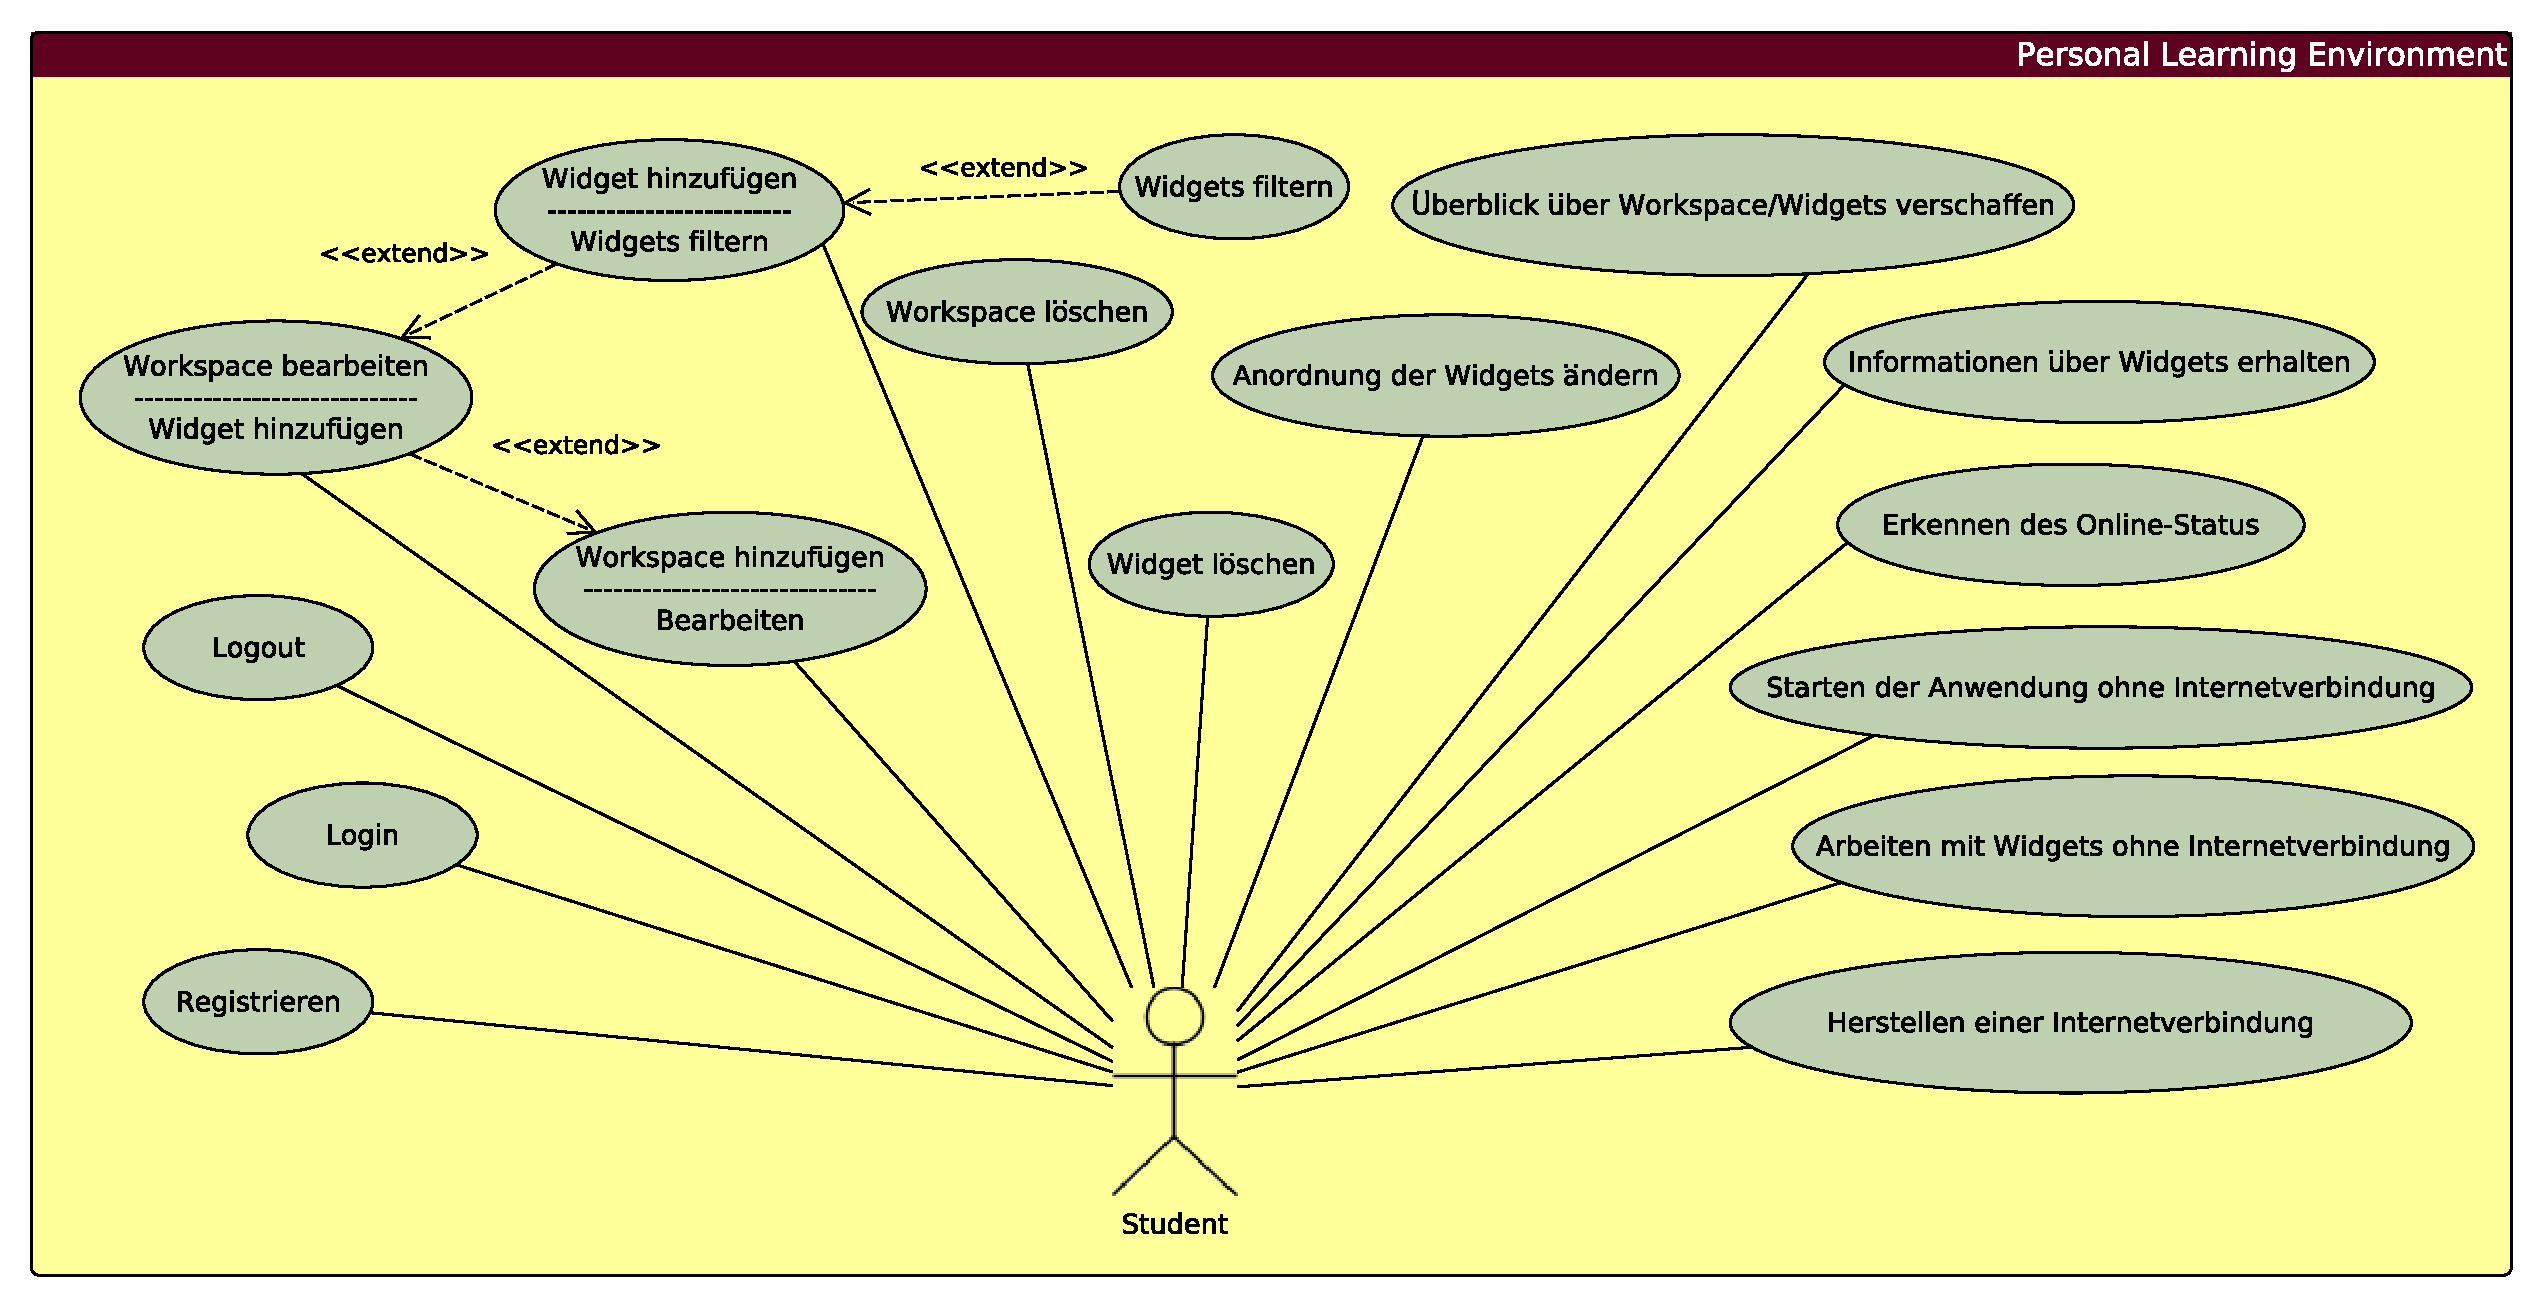
\includegraphics[width=\textwidth,height=\textheight,keepaspectratio]{./Figures/anwendungsfaelle_quer.pdf}
    \rule{35em}{0.5pt}
  \caption[Die wichtigsten Anwendungsfälle für die prototypische Personal Learning EnvironmentAnwendungsfälle der PLE]{Anwendungsfälle der PLE}
  \label{fig:anwendungsfaelle}
\end{figure}

Im folgenden werden die Anwendungsfälle aus Abbildung \ref{fig:anwendungsfaelle} in textueller Form beschrieben. Aus diesen Beschreibungen werden dann direkt die funktionalen Anforderungen an das zu entwickelnde System abgeleitet.

\subsection{Registrieren}
\textbf{use case} \emph{Registrieren}\\
\textbf{actors} Student\\
\textbf{precondition} Das System ist online, der Student ist nicht eingeloggt und es existiert mindestens ein Workspace.\\
\textbf{main flow} Der Student bekommt auf der Startseite die Möglichkeit sich für den Zugang zum System zu registrieren. Er füllt ein Formular mit seinen Daten (Vorname, Nachname, E-Mailadresse, Nutzername, Passwort) aus und schickt das Formular ab.\\
\textbf{postcondition} Der Student ist mit einer Nutzername-/Passwortkombination und seiner E-Mailadresse im System hinterlegt und kann sich somit in das System einloggen.\\
\textbf{exceptional flow} Nutzername oder Mail-Adresse bereits vorhanden. Nutzername und E-Mail-Adresse dürfen nur einmal im System vorkommen.\\
\textbf{postcondition} Der Student bekommt eine Fehlermeldung und muss seine eingetragenen Daten ändern.
 
Aus diesem Anwendungsfall folgt die funktionale Anforderung \emph{fA1}:\\
\emph{fA1: Der Anwender muss sich selbständig in dem registrieren können.}
 
\subsection{Login}
\textbf{use case} \emph{Login}\\
\textbf{actors} Student\\
\textbf{precondition} Das System ist online, der Student ist nicht eingeloggt, ist aber in dem System registriert.\\
\textbf{main flow} Der Student bekommt auf der Startseite die Möglichkeit sich im System anzumelden. Er füllt ein Formular mit seiner Nutzername-/Passwortkombination aus und schickt das Formular ab.\\
\textbf{postcondition} Der Student ist im System eingeloggt und das System präsentiert ihm eine Übersicht über seine aktuellen Workspaces und die wichtigsten aggregierten Informationen dieser.
 
Aus diesem Anwendungsfall folgen die funktionalen Anforderungungen \emph{fA2} und \emph{fA2}:\\
\emph{fA2: Der Anwender muss sich sich in das System mit Nutzername und Passwort einloggen können.}\\
\emph{fA3: Dem Anwender darf nur Zugriff auf die zu seinem Account gehörigen Workspaces und Widgets gewährt werden.}
 
 \subsection{Logout}
\textbf{use case} \emph{Logout}\\
\textbf{actors} Student\\
\textbf{precondition} Das System ist online, der Student ist eingeloggt.\\
\textbf{main flow} Der Student wählt die Aktion "`Logout"' und wird anschließend auf die Login-Seite weitergeleitet.\\
\textbf{postcondition} Die aktuelle Session des Anwenders ist beendet und es ist ohne weiteres Login nicht möglich auf die Daten des Anwenders zuzugreifen 
 
Aus diesem Anwendungsfall folgen die funktionale Anforderung \emph{fA4} und \emph{fA5}:\\
\emph{fA4: Der Anwender muss sich aus dem System ausloggen können.}\\
\emph{fA5: Nach Beendigung der Anwender-Session, darf kein Zugriff mehr auf die Daten des Anwenders bestehen.}
 
\subsection{Workspace hinzufügen}
\textbf{use case} \emph{Workspace hinzufügen}\\
\textbf{actors} Student\\
\textbf{precondition} Das System ist online, der Student ist eingeloggt.\\
\textbf{main flow} Der Student wählt die Aktion "`Workspace hinzufügen"'. Es öffnet sich hierdurch ein neuer Bereich, welcher einen neuen Workspace repräsentiert. Der Student hat nun die Möglichkeit den Workspace nach seinen Wünschen anzupasssen (extension point: Workspace bearbeiten).\\
\textbf{postcondition} Ein neuer Workspace wurde dem System des Studenten hinzugefügt.
 
Aus diesem Anwendungsfall folgt die funktionale Anforderungung \emph{fA6}:\\
\emph{fA6: Der Anwender soll neue Workspaces in seine Lernumgebung einfügen können.}\\
 
\subsection{Workspace bearbeiten}
\textbf{use case} \emph{Workspace bearbeiten}\\
\textbf{actors} Student\\
\textbf{precondition} Das System ist online, der Student ist eingeloggt und es existiert mindestens ein Workspace.\\
\textbf{main flow} Der Student wählt bei einem Workspace die Aktion "`Workspace bearbeiten"'. Der Anwender hat nun die Möglichkeit den Workspace nach seinen Wünschen zu benennen und kann Widgets zu dem Workspace hinzufügen (extension point: Widget hinzufügen).\\
\textbf{postcondition} Der Workspace wurde nach den Vorstellungen des Akteures angepasst.
 
\textbf{extend relationship}\\
\textbf{base} "`Workspace hinzufügen"'\\
\textbf{extensionPoint} Workspace bearbeiten\\
\textbf{extension} "`Workspace bearbeiten"'
 
Aus diesem Anwendungsfall folgt die funktionale Anforderungung \emph{fA7}:\\
\emph{fA7: Der Anwender soll den Namen des Workspaces ändern können.}\\
 
 \subsection{Workspace löschen}
\textbf{use case} \emph{Workspace löschen}\\
\textbf{actors} Student\\
\textbf{precondition} Das System ist online, der Student ist eingeloggt und es existiert mindestens ein Workspace.\\
\textbf{main flow} Der Student wählt bei einem Workspace die Aktion "`Workspace löschen"'. Es erscheint eine Rückfrage, welche eine Bestätigung des Löschvorganges (mitsamt aller Widgets) erfragt. Bei positiver Rückmeldung gibt das System die Nachricht des Löschens aus. \\
\textbf{postcondition} Der Workspace und alle seine Widgets sind aus dem System entfernt.
 
Aus diesem Anwendungsfall folgt die funktionale Anforderungung \emph{fA8}:\\
\emph{fA8: Der Anwender soll einen Workspace löschen können.}\\

\subsection{Widget hinzufügen}
\textbf{use case} \emph{Widget hinzufügen}\\
\textbf{actors} Student\\
\textbf{precondition} Das System ist online, der Student ist eingeloggt und es existiert mindestens ein Workspace.\\
\textbf{main flow} Der Student befindet sich in einem Workspace und wählt die Aktion "`Widget hinzufügen"' Es erscheint eine Maske in der die zur Verfügung stehenden Widgets ausgewählt werden können. Der Student wählt das gewünschte Widget und fügt es dem Workspace hinzu. Wenn gewünscht kann der Student die Liste der Widgets über Suchfilter einschränken (extension point: Widgets filtern)\\
\textbf{postcondition} Das Widget wurde dem Workspace hinzugefügt.
 
\textbf{extend relationship}\\
\textbf{base} `Workspace bearbeiten"'\\
\textbf{extensionPoint} Widget hinzufügen\\
\textbf{extension} "`Widget hinzufügen"'

Aus diesem Anwendungsfall folgt die funktionale Anforderungung \emph{fA9}:\\
\emph{fA9: Der Anwender soll über ein Auswahlfeld Widgets zu Workspaces hinzufügen können.}\\ 

\subsection{Widgets Filtern}
\textbf{use case} \emph{Widgets Filtern}\\
\textbf{actors} Student\\
\textbf{precondition} Der Student ist dabei einem Workspace ein Widget hinzuzufügen.\\
\textbf{main flow} Der Student gibt in einem Textfeld eine Zeichenkette an, nach der im Widgetnamen gesucht wird. Des weiteren kann er in einem binären Filter wählen, ob er nur Widgets angezeigt bekommen möchte, die in der Lage sind in einem Offline-Modus zu arbeiten.\\
\textbf{postcondition} In der Liste der zur Auswahl stehenden Widgets werden nur noch diejenigen angezeigt, die der Filterung entsprechen.
 
\textbf{extend relationship}\\
\textbf{base} "`Widget hinzufügen"'\\
\textbf{extensionPoint} Widgets filtern\\
\textbf{extension} "`Widgets filtern"'
 
Aus diesem Anwendungsfall folgen die funktionale Anforderung \emph{fA10} und \emph{fA11}:\\
\emph{fA10: Der Anwender muss die zur Auswahl stehenden Widgets über ein Suchfeld einschränken können.}\\
\emph{fA11: Der Anwender muss die zur Auswahl stehenden Widgets so einschränken können, dass in der Liste nur offline-fähige Widgets vorkommen.}
 
 \subsection{Widget löschen}
\textbf{use case} \emph{Widget löschen}\\
\textbf{actors} Student\\
\textbf{precondition} Das System ist online, der Student ist eingeloggt, er und es existiert mindestens ein Widget auf einem Workspace.\\
\textbf{main flow} Der Student befindet sich in einem Workspace und wählt bei einem Widget die Aktion "`Widget löschen"'. Es erscheint eine Rückfrage, welche eine Bestätigung des Löschvorganges erfragt. Bei positiver Rückmeldung gibt das System die Nachricht des Löschens aus.
\textbf{postcondition} Das Widget wurde aus dem System entfernt.
 
Aus diesem Anwendungsfall folgt die funktionale Anforderungung \emph{fA12}:\\
\emph{fA12: Der Anwender soll ein Widget löschen können.}\\
 
\subsection{Anordnung der Widgets ändern}
\textbf{use case} \emph{Anordnung der Widgets ändern}\\
\textbf{actors}Student\\
\textbf{precondition} Das System ist online, der Student ist eingeloggt und befindet sich auf der Seite eines Workspaces mit mindestens zwei Widgets.\\
\textbf{main flow} Der Student hat die Möglichkeit die einzelnen Widgets innerhalb eines Workspaces über einen Drag and Drop Mechanismus neu anzuordnen. Er wählt hierfür ein Widget mit der Maus aus und zieht es an die gewünschte Position.\\
\textbf{postcondition} Die Anordnung der Widgets innerhalb des Workspaces hat sich nach dem Wunsch des Studenten geändert.
 
Aus diesem Anwendungsfall folgt die funktionale Anforderungung \emph{fA13}:\\
\emph{fA13: Der Anwender muss in der Lage sein Widgets nach seinen Wünschen über einen Drag and Drop Mechanismus auf dem Workspace zu sortieren .}\\
 
\section{Nichtunktionale Anforderungen}\label{section:nichtfunktionale_anforderunge}
Randbedingungen, umstände etc
 
\section{Zusammenfassung}
Im den vorherigen Abschnitten wurden funktionale und nichtfunktionale Anforderungen an das zu entwickelnde System aufgestellt und beschrieben. In den folgenden zwei Tabellen sind diese Anforderungen noch einmal zusammengefasst.

\renewcommand{\arraystretch}{1.4} 
\begin{table}[h]
\caption{Funktionale Anforderungen}
\begin{tabularx}{\textwidth}{ l | X }
\emph{fA1} & \emph{Der Anwender muss sich selbständig in dem registrieren können.} \\ \hline
\emph{fA2} & \emph{Der Anwender muss sich sich in das System mit Nutzername und Passwort einloggen können.} \\ \hline
\emph{fA3} & \emph{Dem Anwender darf nur Zugriff auf die zu seinem Account gehörigen Workspaces und Widgets gewährt werden.} \\ \hline
\emph{fA4} & \emph{Der Anwender muss sich aus dem System ausloggen können.} \\ \hline
\emph{fA5} & \emph{Nach Beendigung der Anwender-Session, darf kein Zugriff mehr auf die Daten des Anwenders bestehen.} \\ \hline
\emph{fA6} & \emph{Der Anwender soll neue Workspaces in seine Lernumgebung einfügen können.} \\ \hline
\emph{fA7} & \emph{Der Anwender soll den Namen des Workspaces ändern können.} \\ \hline
\emph{fA8} & \emph{Der Anwender soll einen Workspace löschen können.} \\ \hline
\emph{fA9} & \emph{Der Anwender soll über ein Auswahlfeld Widgets zu Workspaces hinzufügen können.} \\ \hline
\emph{fA10} & \emph{Der Anwender muss die zur Auswahl stehenden Widgets über ein Suchfeld einschränken können.} \\ \hline
\emph{fA11} & \emph{Der Anwender muss die zur Auswahl stehenden Widgets so einschränken können, dass in der Liste nur offline-fähige Widgets vorkommen.} \\ \hline
\emph{fA12} & \emph{Der Anwender soll ein Widget löschen können.} \\\hline
\emph{fA13} & \emph{Der Anwender muss in der Lage sein Widgets nach seinen Wünschen über einen Drag and Drop Mechanismus auf dem Workspace zu sortieren .} \\ \hline
\end{tabularx}
\label{table:funktionale_anforderungen}
\end{table}

\section{bla}
Student 1 und Student 2 leben in Kamerun. Beide haben dort das Problem, dass der Internetzugriff aus mehreren Gründen nicht immer gegeben ist. Student 1 hat zu Hause keinen Internetzugang. Er hat nur die Möglichkeit in der Universität oder in einem Internetcafe online zu gehen. Student 2 hat einen Internetzugang, allerdings ist dieser relativ langsam und wird nach Zeit abgerechnet, so dass es vorteilhaft für ihn ist, wenn er nur für kurze Zeit online ist. Aus diesem Grund benötigen die beiden idealerweise ein System, welches ihnen die Möglichkeit bietet die neuesten Informationen auch offline zu lesen und zumindest rudimentär auch offline kleine Aufgaben zu erledigen. Diese sollten sich bei Wiederverbindung mit dem Internet mit den entsprechenden Services synchronisieren. Des Weiteren sollten sie in der Lage sein die Daten auch ohne Internetverbindung zwischen verschiedenen Rechnern auszutauschen. Insbesondere Student 1 sollte in der Lage seine Aktionen bei sich zu Hause vorzunehmen und die durchgeführten Änderungen dann an einem Rechner mit Internetanschluss zu synchronisieren. Die Anforderungen von Student 3 sind ähnlich gelagert. Er ist sehr viel unterwegs und erledigt daher viele kurze Aufgaben mit dem Smartphone. Auch hier ist eine Internetverbindung nicht immer gewährleistet ist oder sie wird temporär deaktiviert um die Akkulaufzeit zu verlängern. Durch die Arbeit an unterschiedlichen Rechnern mit potentiell unterschiedlichen Betriebssystemen, ist die Installation einer komplexen Software nicht ohne Weiteres möglich.

Idealerweise nutzen alle Studenten das selbe Basissystem und können sich hier die benötigten Services und Applikationen so zusammenstellen wie es ihren Ansprüchen entspricht.


Die Arbeit mit einer solchen Lernumgebung kann durch die folgenden Use-Cases beschrieben werden.

Das Ziel der vorliegenden Arbeit ist die Planung und Implementierung eines Prototypen für eine leichtgewichtige Personal-Learning-Environment. Die Anforderungen an das finale System lassen sich aus dem in dem nächsten Abschnitt vorgestellten Use-Case ableiten, welcher die Arbeit mit dem System verdeutlichen soll.

\section{Use Case}
Der folgende Use-Case soll durch das finale System idealerweise abgedeckt werden:

\subsection{Akteure}

\begin{itemize}
 \item Dozent mit Sitz in Hagen
 \item Student 1 mit Sitz in Kamerun (Fernuni Hagen)
 \item Student 2 mit Sitz in Kamerun (Fernuni Hagen)
 \item Student 3 mit Sitz in Berlin (Fernuni Hagen)
 \item Student 4 mit Sitz in Osnabrück (Universität Osnabrück) 
\end{itemize}

\subsection{Ausgangssituation}\label{section:ausgangssituation}
Der Dozent betreut an der Fernuni Hagen unter anderem den Kurs "`E-Learning: A new approach"'. Hierfür haben auch die Studenten 1 und 3 eingeschrieben. Für diesen Kurs hat der Dozent mehrere Kanäle zur Kommunikation angelegt. Die Studenten sollen die Kanäle wählen, die ihren Arbeitsgewohnten am meisten entsprechen. Am Ende des Semesters soll es eine Auswertung geben, welche Kanäle am häufigsten genutzt und welche von den Studenten eher ignoriert wurden. Parallel dazu werden die Systeme der Fernuni zur Online Bearbeitung der Einsendeaufgaben genutzt. Die vom Dozenten angelegten Kommunikationskanäle sind:

\begin{itemize}
 \item ein Twitter Channel
 \item eine Facebookgruppe
 \item einen eigenen Google-Calender
 \item einen Chat
 \item zur Terminabsprache und Abstimmung der nächsten Schritte soll Doodle verwendet werden
 \item ein System zur Hinterlegung von Todo-Listen
 \item einen eigenen Blog, welcher einen RSS Feed bereitstellt 
 \item Etherpad Lite soll zur gemeinsamen Erstellung von Texten genutzt werden
\end{itemize}

Die Studenten sind angehalten sich regelmäßig über Aktualisierungen der Kanäle auf dem Laufenden zu halten.

Zusätzlich haben sich Student 1, 2 und 4 zu einer virtuellen Lerngruppe zum Thema Datenbanken zusammengeschlossen. Hierfür können nicht die Systeme der Fernuni Hagen genutzt werden, da nur Student 2 momentan in dem spezifischen Kurs eingeschrieben ist. Student 1 hat sich nicht für den Kurs angemeldet und Student 4 hat überhaupt keine Möglichkeit dazu, da er nicht an der Fernuni immatrikuliert ist. Sie haben sich dazu entschlossen primär einen Chat zur Kommunikation zu benutzen.

\subsubsection{Einschränkungen/Umstände}
Student 1 und Student 2 leben in Kamerun. Beide haben dort das Problem, dass der Internetzugriff aus mehreren Gründen nicht immer gegeben ist. Student 1 hat zu Hause keinen Internetzugang. Er hat nur die Möglichkeit in der Universität oder in einem Internetcafe online zu gehen. Student 2 hat einen Internetzugang, allerdings ist dieser relativ langsam und wird nach Zeit abgerechnet, so dass es vorteilhaft für ihn ist, wenn er nur für kurze Zeit online ist. Aus diesem Grund benötigen die beiden idealerweise ein System, welches ihnen die Möglichkeit bietet die neuesten Informationen auch offline zu lesen und zumindest rudimentär auch offline kleine Aufgaben zu erledigen. Diese sollten sich bei Wiederverbindung mit dem Internet mit den entsprechenden Services synchronisieren. Des Weiteren sollten sie in der Lage sein die Daten auch ohne Internetverbindung zwischen verschiedenen Rechnern auszutauschen. Insbesondere Student 1 sollte in der Lage seine Aktionen bei sich zu Hause vorzunehmen und die durchgeführten Änderungen dann an einem Rechner mit Internetanschluss zu synchronisieren. Die Anforderungen von Student 3 sind ähnlich gelagert. Er ist sehr viel unterwegs und erledigt daher viele kurze Aufgaben mit dem Smartphone. Auch hier ist eine Internetverbindung nicht immer gewährleistet ist oder sie wird temporär deaktiviert um die Akkulaufzeit zu verlängern. Durch die Arbeit an unterschiedlichen Rechnern mit potentiell unterschiedlichen Betriebssystemen, ist die Installation einer komplexen Software nicht ohne Weiteres möglich.

Idealerweise nutzen alle Studenten das selbe Basissystem und können sich hier die benötigten Services und Applikationen so zusammenstellen wie es ihren Ansprüchen entspricht.

\subsection{Arbeitsabläufe}
Im Folgenden werden die unterschiedlichen Arbeitsabläufe mit dem System exemplarisch an Student 1 und an Student 3 dargelegt.

\subsubsection{Grundsätzlicher Arbeitsablauf für Studenten}
Um mit der PLE arbeiten zu können müssen die Studenten als erstes online eine Account in dem PLE-System erstellen. Anschließend melden sie sich mit ihren gewählten Login-Daten an. Bei erfolgreicher Anmeldung hat der Anwender die Möglichkeit direkt Workspaces zu erstellen, mit diesen zu arbeiten (Workspace umbenennen, Einstellungen vornehmen, Widgets hinzufügen etc).

\subsubsection{Arbeitsablauf Student 1}
\begin{itemize}
 \item \emph{Tag 1:} Student 1 befindet sich in der Universität und verbindet seinen USB-Stick mit einem PC. Auf diesem Stick befindet sich die ausführbare mobiler Version eines aktuellen Browsers. Er öffnet die Applikation online in diesem Browser (alle folgenden Aktionen werden mit dem selben Browser durchgeführt). Student 1 erstellt einen neuen Workspace und benennt ihn in "`PLE"' um. Anschließend sucht er die Widgets für den PLE Workspace aus der Widget-Datenbank heraus. Das System zeigt ihm dabei an, für welche Widgets eine Offline-Fähigkeit zur Verfügung steht. Daraufhin organisiert er die Anordnung der Widgets nach seinen Vorstellungen per Drag and Drop neu. Damit er mit den einzelnen Widgets auch arbeit kann meldet sich Student 1 schließlich bei den jeweiligen Services mit seinen Account-Daten an. Bevor er den Browser schließt haben sich alle Widgets mit ihren Services synchronisiert und zeigen ihm dies auch an.
 \item \emph{Tag 2:} Student 1 loggt sich an der Uni in das PLE-System ein. Das System zeigt ihm auf der Startseite (dem Dashboard) an wie viele neue Items es auf seinem PLE Workspace gibt. Ein direkter Link führt ihn zum Workspace. Er sieht, dass momentan mehrere Leute im Chat sind und unterhält sich über das Widget mit ihnen. Der Dozent hat einige globale Todos angelegt und die ersten Nachrichten kommen über den Twitter Channel herein. Nach einiger Zeit klickt Student 1 auf “jetzt offline gehen” wodurch alle Widgets seines Workspaces auf den neuesten Stand gebracht werden. Er sieht, dass Student 3 einen längeren Text im Chat geschrieben hat, beschließt diesen jedoch später zu lesen. Gleiches gilt für den Einführungsartikel des Dozenten im Kursblog. Hierfür erstellt er sich Items in seiner Todo-Liste. Abschließend schließt Student 1 den Browser und entfernt den USB-Stick.
 \item \emph{Tag 3:} Student 1 öffnet die Applikation in seinem mobilen Browser zu Hause. Das System erkennt, dass es sich im Offline-Modus befindet und versucht keine Synchronisierung mit dem Internet herzustellen. Student 1 liest den Text, den Student 3 im Chat hinterlegt hat und beantwortet die darin gestellten Fragen ebenfalls im Chatfenster. Anschließend teilt er dies über Twitter mit und erledigt sein Todo-Item.
 \item \emph{Tag 4:} Student 1 loggt sich im Internet-Cafe mit seinem mobilen Browser in das System ein. Das System erkennt, dass es online ist, lädt die neuesten Items der Services herunter und synchronisiert die nur lokal vorgenommenen Aktionen (Twitter, Chat, Todo). Per Mail hat Student 1 den Vorschlag von Student 2 bekommen gemeinsam mit Student 4 eine Lerngruppe zum Thema Datenbanken zu gründen. Hierzu wollen sie unter anderem ein Chat-System benutzen. Student 1 schlägt per Mail das ihm bekannte Chat-Widget für die PLE-Applikation vor. Er erstellt einen neuen Workspace, nennt ihn “Lerngruppe DB” und fügt das Chat-Widget mit den passenden Einstellungen hinzu.
 \item \emph{Tag 5:} Student 1 sieht in seinem Dashboard, dass es für den Workspace “Lerngruppe DB” 12 neue Items gibt. Er geht direkt zu dem Workspace und stellt fest, dass die beiden anderen Studenten sich ebenfalls in dem Chat angemeldet haben. Da momentan alle online verfügbar sind, beginnen sie ihre erste Gruppenunterhaltung und planen die weitere Vorgehensweise.
\end{itemize}

\subsubsection{Arbeitsablauf Student 3}
Student 3 nutzt das System hauptsächlich mit seinem Tablet, welches in der Lage ist sich über Wlan, sowie UMTS mit dem Internet zu verbinden.

\begin{itemize}
 \item \emph{Tag 1:} Student 3 meldet sich ähnlich wie Student 1 in der PLE an und erstellt für seine Uni-Kurse jeweils einen Workspace. Außerdem legt er sich einen Workspace an, in dem sich nicht kursspezifische Widgets finden. Hierzu gehören sein Google-Kalender, sein RSS-Reader, eine Todo Liste, sowie ein News-Widget
 \item \emph{Tag 2:} Student 3 verbindet sich zu Hause mit seinem Wlan und loggt sich in der PLE ein. Nach Prüfung des Dashboards erstellt er sich in der allgemeinen Todo Liste für den Tag. Er sieht, dass es in seinem RSS-Reader 9 neue Artikel gibt. Diese möchte er auf seinem Weg zur Uni in der U-Bahn lesen. Da dort der Empfang eher schlecht ist, synchronisiert er die PLE noch einmal. Auf dem Weg zu Uni ruft Student 3 das System auf seinem Tablet auf. Da kein Internetzugang besteht greift das System nur auf die lokalen Daten zurück. Das News-Widget in seinem globalen Workspace ist nicht offline-fähig. Aus diesem Grund wird es auch nur ausgegraut und nicht-funktional angezeigt. Der Student ist jedoch in der Lage seine lokal gecachten RSS-Artikel zu lesen. Bei Lektüre eines Artikels über Javascript fällt ihm ein, dass er sein Uni-Projekt noch mit der neuesten JQuery Version updaten wollte. Hierzu erstellt er sich ein weiteres Todo auf seiner Liste.
 In der Uni verbindet er sein Tablet mit dem Uni-Wlan. Der RSS-Reader markiert die 6 Artikel die, Student 3 in der U-Bahn gelesen hat als gelesen und synchronisiert das neueste Todo-Item mit dem Service im Internet.  
\end{itemize}

\section{Anforderungen}\label{section:anforderungen_summary}
Zusammenfassend kann also gesagt werden, dass Betreuer und Studenten stehen über unterschiedliche Kanäle in Kommunikation miteinander stehen. Es müssen Termine geplant oder auch Notizen und Nachrichten hin und hergeschickt werden. Diese Kanäle sollen auf einem zentralen Zugang so zusammengefasst sein, dass es den Teilnehmern des Kurse alle relevanten Informationen an einer aufrufen und bearbeiten zu können. Dabei sind die Teilnehmer zu unterschiedlichen Zeiten online. Die Teilnehmer sollen das System offline Nutzen können, um einfache Arbeiten wie das Schreiben von Twitter-Nachrichten, Notizen und Instant-Messaging Nachrichten oder eine Terminabsprache über einen Kalender erledigen können. Bei dem Wechsel zwischen Online und Offline müssen die Daten synchronisiert werden. Idealerweise haben die Nutzer alle Daten auf einem USB-Stick bei sich und können so von unterschiedlichsten Rechnern, wie beispielsweise in der Universität, im Internetcafe oder zu von Hause aus, arbeiten.

Daraus lassen sich mehrere Anforderungen an das zu entwickelnde System ableiten. Es soll in der Lage sein als Aggregator für die unterschiedlichsten Services und Kanäle zu dienen. Es muss möglich sein auf die wichtigsten Informationen an einem zentralen Platz zuzugreifen und diese auch zu bearbeiten (Anforderung 1). Dadurch, dass die Teilnehmer an unterschiedlichen Rechnern arbeiten, welche zum Teil nicht in ihrem persönlichen Besitz sind, ist es für sie nicht oder nur sehr schwer möglich eine neue Software zu installieren. Aus diesem Grund soll das System mit nativen Browsertechnologien ohne weitere Installation nutzbar sein (Anforderung 2). Das System muss in der Lage die wichtigsten Funktionalitäten auch dann zu Verfügung zu stellen, wenn es keinen Kontakt zu dem Internet hat (Anforderung 3). Des Weiteren soll es in der Lage sein bei einer Wiederaufnahme der Verbindung die durchgeführten Aktionen mit dem jeweiligen Service zu synchronisieren (Anforderung 4). Dies gilt insbesondere für die Arbeit mit unterschiedlichen Rechnern. Der Nutzer soll sein System an einem Computer mit dem Internet synchronisieren können und dann an einem anderen Rechner offline weiterarbeiten können. Es ist also notwendig, dass es dem Nutzer ermöglicht wird die Daten mitzunehmen (beispielsweise per USB-Stick) und an anderer Stelle weiterzuverwenden (Anforderung 5). 

Neben diesen funktionalen Anforderungen gibt es noch weitere Anforderungen, welche das System erfüllen soll. In dieser Arbeit kann nur eine prototypische Implementierung der Anforderungen erfolgen. Das System soll also als Basis für weitere Entwicklungen und Forschungsarbeiten dienen und einfach erweitert und verändert werden können (Anforderung 6). Es soll auch möglich sein auf Basis einer vorgegebenen Implementierung oder API weitere Services oder Kanäle in das System zu laden und es so beständig in seiner Funktionalität zu erweitern (Anforderung 7). Schließlich wird die Software in unterschi Bereichen, insbesondere in einem universitären Umfeld eingesetzt. Dies verlangt eine Nutzbarkeit ohne Lizengebühren für die genutzten Technologien. Daraus folgt, dass für die Umsetzun keine proprietären, sondern nur freie Technologien verwendet werden dürfen (Anforderung 8). 

\begin{table}[h]
\caption{Anforderungen}
\begin{tabular}{c || l}
1 & Informationsaggregator \\
\hline
2 & ohne Installationsaufwand lauffähig in aktuellen Browsern \\
\hline
3 & Möglichkeit des (zumindest rudimentären) Weiterarbeitens, wenn offline \\
\hline
4 & Synchronisierung der vorgenommen Änderungen, wenn wieder online \\
\hline
5 & Daten können zwischen unterschiedlichen Rechnern offline ausgetauscht werden \\
\hline
6 & kann als Basis für weitere Entwicklungen dienen\\
\hline
7 & neue Services und Kanäle sollen sich einfach in das System integrieren lassen  \\
\hline
8 & ausschließliche Verwendung freier Technologien \\
\hline
\end{tabular}
\label{table:anforderungen}
\end{table}

Die in Abschnitt \ref{section:ausgangssituation} beschriebenen Kanäle und Services müssen für eine vollständige PLE implementiert werden. Da die Umsetzung all dieser aber den Rahmen dieser Arbeit übersteigen würde und das Ziel ist einen Prototypen für die Grundlage einer solchen PLE zu schaffen, werden diese nicht in die Anforderungen aufgenommen.